\documentclass[10pt,conference]{IEEEtran}
\IEEEoverridecommandlockouts

\usepackage{cite}
\usepackage{amsmath,amssymb,amsfonts}
\usepackage{algorithmic}
\usepackage{graphicx}
\usepackage{textcomp}
\usepackage{xcolor}
\usepackage{booktabs}
\usepackage{multirow}
\usepackage{url}
\usepackage{tikz}
\usepackage{pgfplots}
\pgfplotsset{compat=1.17}
\usetikzlibrary{patterns,shadows,shapes,arrows}

% Define IEEE-compliant professional colors
\definecolor{ieeeblue}{RGB}{0,101,189}
\definecolor{ieeered}{RGB}{215,25,32}
\definecolor{ieeegreen}{RGB}{0,146,69}
\definecolor{ieeeorange}{RGB}{237,139,0}
\definecolor{ieeegray}{RGB}{128,128,128}
\definecolor{ieeelight}{RGB}{245,245,245}
\definecolor{ieeeyellow}{RGB}{255,204,0}

% Set IEEE-compliant plot defaults
\pgfplotsset{
    compat=newest,
    % Default axis style
    every axis/.append style={
        width=\columnwidth,
        height=0.65\columnwidth,
        scale only axis,
        % Fonts
        tick label style={font=\footnotesize},
        label style={font=\small},
        legend style={font=\footnotesize,draw=black,fill=white,fill opacity=0.9},
        title style={font=\normalsize},
        % Lines
        axis line style={line width=0.5pt},
        major tick style={line width=0.5pt},
        minor tick style={line width=0.25pt},
        % Grid
        grid=major,
        major grid style={line width=0.25pt,draw=gray!50,dashed},
        minor grid style={line width=0.15pt,draw=gray!20,dotted},
        % Ticks
        xtick align=outside,
        ytick align=outside,
        % Legend
        legend cell align={left},
        legend pos=north east,
    },
    % Line plot style
    every axis plot/.append style={
        line width=1.25pt,
        mark size=2.5pt,
        mark options={solid,fill=white,line width=0.75pt}
    },
}
\def\BibTeX{{\rm B\kern-.05em{\sc i\kern-.025em b}\kern-.08em
    T\kern-.1667em\lower.7ex\hbox{E}\kern-.125emX}}

\begin{document}

\title{Best-of-Breed, Worst-of-System: How AI Excellence Creates Security Disasters}

\author{\IEEEauthorblockN{Manish Bhatt}
\IEEEauthorblockA{\textit{AI Offensive Security Researcher} \\
\textit{OWASP/Project Kuiper}\\
manish.bhatt13212@gmail.com}
\and
\IEEEauthorblockN{Idan Habler}
\IEEEauthorblockA{\textit{Adversarial AI Security reSearch} \\
\textit{Intuit}\\
idan\_habler@intuit.com}}

\maketitle

\begin{abstract}
Security folks increasingly rely on AI-driven agents to manage the overwhelming volume of security alerts. Industry practice favors procuring ``best-of-breed'' solutions---agents that excel at specific metrics such as speed, accuracy, or resource efficiency. Through comprehensive Monte Carlo simulation of 40,000 security incidents across 11 distinct optimization strategies, we demonstrate that this procurement approach creates catastrophic system-level failures. Our simulation incorporates adaptive adversary dynamics where poor defense strategies trigger increased attack rates, creating realistic but varying threat environments. Under these conditions, failed single-metric strategies faced up to 3,200+ attacks while the balanced approach suppressed threats to just 455 attacks. Our findings reveal that 7 out of 11 single-metric optimization strategies detect zero attacks, while a balanced multi-objective approach achieves 94.5\% detection rates. We formalize this phenomenon as the ``best-of-breed optimization paradox'' and provide empirical evidence that hyper-optimization for individual metrics creates exploitable blind spots that adversaries leverage. Our work introduces a $\gamma$-parameterized reward shaping framework that aligns agent incentives with organizational security objectives, achieving 12$\times$ improvement in utility compared to single-metric approaches. These results challenge fundamental assumptions about AI procurement in security and provide a quantitative framework for building resilient, integrated security systems.
This paper outlines a footgun, and formalizes it as a way to incorrectly make agentic systems.
\end{abstract}

\begin{IEEEkeywords}
Security Operations, AI Agents, Optimization Paradox, Multi-objective Optimization, Security Analytics, Best-of-Breed, System Integration
\end{IEEEkeywords}

\section{Introduction}

The modern Security Practice faces an existential challenge: processing millions of security events daily while maintaining near-perfect detection of genuine threats. The sheer volume of data has made human-only analysis infeasible, driving widespread adoption of AI-driven security agents. These agents promise to automate triage, reduce analyst workload, and improve response times---critical metrics in an environment where minutes can mean the difference between a contained incident and a catastrophic breach.

The security industry has responded to this challenge by developing specialized AI agents, each optimized for specific performance metrics. Speed-optimized agents boast sub-second triage times. Accuracy-focused solutions claim 99.9\% precision rates. Resource-efficient agents minimize computational overhead. User experience champions promise frictionless security. This specialization has created a marketplace where vendors compete on narrow benchmarks, and procurement teams assemble ``best-of-breed'' stacks by selecting the top performer in each category.

This procurement strategy appears logical: if each component is best at its designated task, surely their combination yields the best overall system. We term this the ``best-of-breed assumption''---the belief that excellence in components translates to excellence in systems. Through rigorous empirical analysis, we demonstrate this assumption is not merely wrong but catastrophically so. Single-metric optimization doesn't just degrade system performance; it creates complete security failures.

\subsection{The Hidden Cost of Optimization}

Consider a speed-optimized triage agent trained to minimize mean time to decision (MTTD). To achieve benchmark-leading performance, the agent learns the fastest path: dismiss everything. After all, dismissing an alert takes 0.5 seconds while investigating requires 5--30 minutes. From a pure speed perspective, the agent performs perfectly---processing thousands of alerts per second with zero queue buildup. From a security perspective, it's a disaster, missing every attack.

This pattern extends beyond speed. An accuracy-optimized agent, trained to minimize false positives, sets its detection threshold so high that only unmistakable attacks trigger alerts. While achieving 99.9\% precision, it misses sophisticated threats that don't match known patterns perfectly. A resource-efficiency champion performs shallow analysis to minimize CPU usage, missing multi-stage attacks that require correlation. Each optimization creates its own failure mode.

\subsection{The Paradox Emerges}

The best-of-breed optimization paradox emerges from a fundamental mismatch between component metrics and system objectives. Security isn't about speed, accuracy, or efficiency in isolation---it's about detecting and responding to threats while maintaining operational viability. When agents optimize for proxy metrics rather than actual security outcomes, they create predictable patterns that adversaries exploit.

Our research quantifies this paradox through large-scale simulation. We implement 11 distinct optimization strategies representing common procurement criteria and evaluate their performance on 40,000 security incidents. The results are stark: 7 out of 11 strategies achieve 0\% detection rates, catching zero attacks out of thousands. Even ``successful'' single-metric approaches like compliance (45.4\% detection) or coverage (44.8\% detection) miss the majority of threats.

\subsection{Contributions and Paper Organization}

This paper makes four primary contributions to the field of AI security systems:

\textbf{1. Formalization of the Optimization Paradox:} We provide the first formal characterization of how single-metric optimization creates system-level security failures, establishing a theoretical framework for understanding component-system misalignment.

\textbf{2. Comprehensive Empirical Evidence:} Through Monte Carlo simulation of 40,000 incidents across 11 optimization strategies, we quantify the paradox's impact, demonstrating that best-of-breed procurement strategies lead to catastrophic failure modes.

\textbf{3. Multi-Objective Solution Framework:} We introduce a $\gamma$-parameterized reward shaping approach that aligns agent behavior with organizational security objectives, achieving 94.5\% detection rates while maintaining operational efficiency.

\textbf{4. Industry Guidance:} We provide actionable recommendations for security leaders, vendors, and researchers on moving beyond single-metric optimization toward integrated, resilient security systems.

The remainder of this paper is organized as follows. Section II reviews related work in AI security systems, multi-objective optimization, and system integration challenges. Section III formalizes the optimization paradox and presents our theoretical framework. Section IV details our simulation methodology and experimental design. Section V presents comprehensive results demonstrating the paradox across multiple dimensions. Section VI analyzes why best-of-breed fails and how our solution succeeds. Section VII discusses implications for industry practice. Section VIII provides broader discussion of theoretical and practical significance. Section IX outlines future research directions. Finally, Section X concludes with key takeaways and a call to action for the security community.

\section{Related Work}

The best-of-breed optimization paradox sits at the intersection of several research domains: AI agent design, security operations optimization, multi-objective decision making, and system integration theory. We review relevant work in each area to contextualize our contributions.

\subsection{AI Agents in Security Operations}

The application of AI to security operations has accelerated dramatically in recent years. Chen et al. \cite{chen2022ai} provide a comprehensive survey of AI techniques in SOCs, categorizing approaches by their primary optimization target. They identify speed, accuracy, and resource efficiency as the dominant metrics but note that ``real-world performance often falls short of laboratory benchmarks.'' Our work explains why: laboratory benchmarks measure component performance, not system effectiveness.

Liu and Zhang \cite{liu2023speed} specifically examine speed-optimized triage agents, achieving sub-second classification times through aggressive feature reduction. While impressive in isolation, they acknowledge ``occasional misses of complex attacks.'' Our simulations reveal these aren't occasional misses but systematic failures---speed optimization drives detection rates to zero.

Johnson et al. \cite{johnson2024accuracy} pursue the opposite approach, developing high-precision detection models that minimize false positives. Their agent achieves 99.97\% precision but requires 45 minutes per alert for deep analysis. In a SOC processing thousands of daily alerts, such an agent becomes operationally infeasible, creating massive backlogs that ironically reduce security by delaying response to critical threats.

\subsection{Multi-Objective Optimization in Security}

The tension between competing objectives in security systems has long been recognized. Gordon and Loeb \cite{gordon2002economics} established the economic framework for security investment, showing that optimal spending depends on vulnerability, threat frequency, and potential loss. However, their model assumes agents can be directly programmed with these trade-offs, not that they're procured based on single metrics.

Kwon and Johnson \cite{kwon2021multi} explore multi-objective optimization for intrusion detection, using Pareto frontiers to balance detection rate against false positive rate. While valuable, their approach assumes a single, integrated system rather than a collection of best-of-breed components. They don't address how individually optimized agents interact when combined.

Recent work by Patel et al. \cite{patel2024reward} introduces reward shaping for security agents, showing that appropriate incentive structures can align agent behavior with organizational goals. Our $\gamma$-parameterized approach builds on this foundation but specifically addresses the best-of-breed problem by providing a unifying framework across diverse optimization targets.

\subsection{System Integration and Emergent Failures}

The challenges of integrating specialized components into effective systems extend beyond security. Leveson \cite{leveson2011engineering} pioneered the study of system safety, showing how component reliability doesn't guarantee system reliability. She identifies ``component interaction accidents'' where individually correct components create system failures through their interaction. The best-of-breed optimization paradox represents a specific instance of this phenomenon.

In the AI domain, Amodei et al. \cite{amodei2016concrete} catalog problems in AI safety, including ``reward hacking'' where agents achieve high scores on metrics while violating their intended purpose. Our speed-optimized agents that dismiss all alerts exemplify this behavior---perfect MTTD scores, zero security value.

Marcus and Davis \cite{marcus2019rebooting} argue that current AI systems are ``brittle'' because they optimize for narrow objectives without understanding broader context. In security, this brittleness manifests as agents that excel at benchmarks while failing at their fundamental purpose: protecting organizations from threats.

\subsection{Security Operations Research}

The operational challenges of modern SOCs are well-documented. Sundaramurthy et al. \cite{sundaramurthy2016anthropological} conducted ethnographic studies of SOC analysts, finding that tool proliferation creates ``swivel chair'' workflows where analysts constantly switch between specialized systems. Best-of-breed procurement exacerbates this problem by maximizing the number of distinct, non-integrated components.

Bhatt et al. \cite{bhatt2014economics} examine the economics of SOC operations, showing that investigation costs dominate operational expenses. They propose automation to reduce these costs but don't address how optimization for cost reduction might compromise security effectiveness. Our results show cost optimization performs better than most single metrics but still misses 10\% of attacks.

Recent industry reports \cite{ponemon2024soc} indicate that 75\% of organizations use 10+ security tools, with integration challenges cited as the primary operational pain point. Our work suggests the problem isn't just integration complexity but fundamental incompatibility between components optimized for different objectives.

\subsection{Theoretical Foundations}

The optimization paradox connects to broader theoretical frameworks in several ways:

\textbf{Goodhart's Law:} ``When a measure becomes a target, it ceases to be a good measure'' \cite{goodhart1984problems}. In security, when MTTD becomes the target, agents optimize for speed at the expense of actual threat detection.

\textbf{Principal-Agent Theory:} Jensen and Meckling \cite{jensen1976theory} show how misaligned incentives create suboptimal outcomes. In our context, the ``principal'' (organization) wants security, but ``agents'' (AI systems) are incentivized by their training metrics.

\textbf{Systems Thinking:} Meadows \cite{meadows2008thinking} emphasizes that system behavior emerges from component interactions, not just component properties. The best-of-breed approach violates this principle by assuming component excellence ensures system excellence.

\subsection{Gap in Existing Literature}

While prior work addresses pieces of the puzzle---multi-objective optimization, system integration challenges, SOC operations---none directly confronts the best-of-breed optimization paradox. Existing research either:
\begin{itemize}
\item Assumes integrated systems where trade-offs can be centrally managed
\item Focuses on single-agent optimization without considering ensemble effects
\item Addresses operational challenges without examining their root cause in procurement strategies
\end{itemize}

Our work fills this gap by:
\begin{itemize}
\item Formalizing how single-metric optimization creates system failure
\item Quantifying the paradox across multiple optimization targets
\item Providing a solution framework that aligns component behavior with system objectives
\item Offering empirical evidence from large-scale simulation
\end{itemize}

This comprehensive approach reveals that the best-of-breed optimization paradox isn't a minor inefficiency but a fundamental flaw in how the industry approaches AI security systems.

\section{Formalizing the Optimization Paradox}

To understand why best-of-breed procurement fails, we must first formalize the decision-making process in security operations and show how single-metric optimization creates systematic vulnerabilities.

\subsection{The Security Decision Model}

We model security operations as a sequential decision process where agents must classify incoming alerts as benign or malicious. Let:

\begin{itemize}
\item $H \in \{0, 1\}$ represent the true state (benign/malicious)
\item $E \in \mathcal{E}$ represent observable evidence
\item $A \in \{\text{dismiss}, \text{investigate}\}$ represent available actions
\item $\pi = P(H = 1)$ represent the prior probability of malicious activity
\end{itemize}

The agent's task is to compute the posterior probability $P(H = 1 | E)$ and decide whether investigation is warranted.

\subsection{Cost Structure and Utility Function}

Security operations incur both time costs (operational overhead) and monetary losses (from missed attacks). We unify these into a single utility metric:

$$U = -\sum_{i} c_{\text{time}}(a_i) - \sum_{j} L_j \cdot \mathbb{I}[\text{attack}_j \text{ missed}]$$

where time costs are converted to monetary equivalents using $\$100/\text{hour}$ (typical SOC analyst rate), and breach losses follow a heavy-tailed distribution. The term $\Delta U$ in the balanced objective represents the expected change in global utility from taking action $a$.

\begin{table}[!h]
\centering
\caption{Action Costs and Loss Distribution}
\begin{tabular}{@{}lcc@{}}
\toprule
\textbf{Action/Event} & \textbf{Time Cost} & \textbf{Monetary Equivalent} \\
\midrule
Dismiss alert & 0.5 minutes & \$0.83 \\
Initial triage & 1.0 minute & \$1.67 \\
Automated investigation & 5.0 minutes & \$8.33 \\
Manual investigation & 30.0 minutes & \$50.00 \\
\midrule
\multicolumn{3}{l}{Missed attack loss: $L \sim \text{LogNormal}(\mu=6, \sigma=1.2)$ (mean = \$828)} \\
\bottomrule
\end{tabular}
\end{table}

\subsection{Optimization Targets}

We formalize 11 distinct optimization strategies. For single-metric strategies, we model their behavior through investigation thresholds that reflect their optimization focus:

\begin{table*}[h]
\centering
\caption{Optimization Strategies: Objectives and Implementation}
\footnotesize
\begin{tabular}{@{}lllc@{}}
\toprule
\textbf{Strategy} & \textbf{Objective} & \textbf{Implementation} & \textbf{Threshold} \\
\midrule
Speed & Minimize time per incident & Never investigate & $\theta = 1.0$ \\
Accuracy & Maximize precision & Only near-certain threats & $\theta = 0.95$ \\
False Positive Min. & Minimize false alarms & Extreme caution & $\theta = 0.98$ \\
Resource Efficiency & Minimize computation & Quick decisions only & $\theta = 0.85$ \\
Alert Volume & Reduce workload & Minimize investigations & $\theta = 0.90$ \\
Compliance & Meet regulations & Fixed 10\% random sampling & N/A \\
User Experience & Minimize disruption & Avoid business hours & N/A \\
Cost & Minimize monetary cost & Balance time vs loss & $\theta = 0.65$ \\
Coverage & Detect all threat types & Cast wide net & $\theta = 0.45$ \\
Automation & Maximize automation & No human escalation & $\theta = 1.0$ \\
\rowcolor{ieeegreen!10}
\textbf{Balanced} & \textbf{Multi-objective} & \textbf{Adaptive threshold} & $\boldsymbol{\theta = \frac{0.7}{1 + 10\gamma}}$ \\
\bottomrule
\end{tabular}
\end{table*}

where $\theta$ represents the posterior probability threshold for investigation: $P(H=1|E) > \theta$.

\subsection{The Paradox Mechanism}

The optimization paradox arises because each single-metric optimization creates a decision boundary that adversaries can exploit:

\begin{theorem}
For any single-metric optimization $f: \mathcal{A} \to \mathbb{R}$, there exists an adversarial strategy $s^*$ such that an agent optimizing $f$ achieves arbitrarily poor security outcomes while maintaining optimal $f$ scores.
\end{theorem}

\begin{proof}
Consider speed optimization where $f(a) = -\text{time}(a)$. The optimal policy $\pi^*_f$ minimizes time by setting $P(\text{investigate} | E) = 0$ for all $E$. An adversary observing this policy can execute any attack with probability 1 of success, while the agent maintains perfect speed scores.

This generalizes: for any metric $f$ not directly measuring security outcomes, the optimal policy $\pi^*_f$ creates predictable behavior that adversaries exploit. The agent achieves $f^* = \max f$ while security utility $U \to -\infty$.
\end{proof}

\subsection{Emergent System Failures}

When multiple best-of-breed agents combine, the failure modes compound:

\begin{itemize}
\item \textbf{Coverage Gaps:} Each agent's blind spots create system-wide vulnerabilities
\item \textbf{Conflicting Decisions:} Agents optimized for different metrics disagree, creating deadlock
\item \textbf{Cascade Failures:} One agent's optimization undermines another's effectiveness
\item \textbf{Integration Overhead:} Coordination costs eliminate efficiency gains
\end{itemize}

The result is a system that performs worse than any individual component---the opposite of the intended outcome.

\section{Methodology}

To empirically validate the optimization paradox, we developed a comprehensive simulation framework modeling realistic SOC operations with multiple optimization strategies.

\subsection{Simulation Architecture}

\begin{table}[!h]
\centering
\caption{Simulation Parameters and Dynamics}
\footnotesize
\begin{tabular}{@{}ll@{}}
\toprule
\textbf{Component} & \textbf{Specification} \\
\midrule
\multicolumn{2}{l}{\textit{Incident Generation}} \\
Arrival process & Poisson, $\lambda = 40$ per hour \\
Base malicious rate & $\pi = 0.02$ (2\%) \\
\midrule
\multicolumn{2}{l}{\textit{Evidence Model}} \\
Evidence levels & $E \in \{\text{Low, Medium, High}\}$ \\
$P(E = \text{High} | \text{malicious})$ & 0.8 \\
$P(E = \text{High} | \text{benign})$ & 0.1 \\
\midrule
\multicolumn{2}{l}{\textit{Dynamic Elements}} \\
Adaptive base rate & $\pi \to 0.1$ if dismiss rate $> 90\%$ \\
Adversary evolution & Stealth $+3\%$/batch if dismiss $> 80\%$ \\
Queue cost scaling & $c = c_{base}(1 + 0.5 \cdot \text{queue}/\text{capacity})$ \\
Loss distribution & LogNormal($\mu=6, \sigma=1.2$) \\
\bottomrule
\end{tabular}
\end{table}

\subsection{Implementation Details}

Each optimization strategy is implemented through a decision function that computes the investigation probability based on evidence strength. We use Bayesian inference to compute posterior probabilities:

$$P(H=1|E) = \frac{P(E|H=1) \cdot \pi}{P(E|H=1) \cdot \pi + P(E|H=0) \cdot (1-\pi)}$$

The strategies differ in how they use this posterior:

\begin{itemize}
\item \textbf{Speed/Alert Volume/Automation}: Always dismiss ($P(\text{investigate}) = 0$)
\item \textbf{Accuracy}: Investigate only if $P(H=1|E) > 0.95$
\item \textbf{False Positive Min}: Investigate only if $P(H=1|E) > 0.98$
\item \textbf{Resource Efficiency}: Quick check only, investigate if $P(H=1|E) > 0.85$ and queue small
\item \textbf{Compliance}: Fixed 10\% random sampling regardless of evidence
\item \textbf{Coverage}: Low threshold, investigate if $P(H=1|E) > 0.45$
\item \textbf{Cost}: Dynamic threshold based on expected loss vs investigation cost
\item \textbf{User Experience}: Avoid investigations during business hours (8am-6pm)
\item \textbf{Balanced}: Adaptive threshold $\theta = \frac{0.7}{1 + 10\gamma}$
\end{itemize}

We simulate 40,000 incidents for each strategy, tracking detection performance, operational metrics, and economic outcomes. The key innovation is allowing adversaries to adapt their behavior based on observed defender actions.

\subsection{Statistical Analysis}

With $\pi = 0.02$ and 40,000 incidents, we expect approximately 800 malicious incidents (95\% CI: [765, 835]). This provides sufficient statistical power to detect meaningful differences between strategies.

We use:
\begin{itemize}
\item Chi-squared tests for comparing detection rates
\item Cohen's d for effect sizes
\item Bootstrap confidence intervals for utility estimates
\end{itemize}

\subsection{Validation}

To ensure simulation fidelity, we:
\begin{itemize}
\item Calibrated parameters against industry reports \cite{verizon2024dbir}
\item Validated queue dynamics with SOC operational data
\item Confirmed loss distributions match breach cost studies
\item Tested sensitivity to parameter variations
\end{itemize}

\section{Results}

Our simulation results provide definitive evidence of the best-of-breed optimization paradox across multiple dimensions.

\subsection{Primary Findings}

Our results reveal three distinct performance categories. Critically, the adaptive adversary dynamics mean that different strategies faced vastly different threat environments, amplifying the consequences of poor optimization choices:

\begin{table*}[!ht]
\centering
\caption{Performance Metrics Across Optimization Strategies (40,000 Incidents, Adaptive Attack Rates)}
\label{tab:main_results}
\renewcommand{\arraystretch}{1.2}
\footnotesize
\begin{tabular}{@{}lcccccccl@{}}
\toprule
\textbf{Optimization} & \textbf{Detection} & \textbf{Caught} & \textbf{Missed} & \textbf{Total} & \textbf{Avg Utility} & \textbf{Time/Inc} & \textbf{Inv. Rate} & \textbf{Performance} \\
\textbf{Strategy} & \textbf{Rate (\%)} & \textbf{Attacks} & \textbf{Attacks} & \textbf{Attacks} & \textbf{(per incident)} & \textbf{(minutes)} & \textbf{(\%)} & \textbf{Category} \\
\midrule
\rowcolor{ieeelight}
\multicolumn{8}{l}{\textit{Complete Failures -- Zero Detection Capability}} \\
Speed & 0.0 & 0 & 3,153 & 3,153 & $-65.01$ & 0.50 & 0.0 & \cellcolor{red!20}Catastrophic \\
Accuracy & 0.0 & 0 & 3,120 & 3,120 & $-66.08$ & 0.50 & 0.0 & \cellcolor{red!20}Catastrophic \\
False Positive Min. & 0.0 & 0 & 3,054 & 3,054 & $-65.66$ & 0.50 & 0.0 & \cellcolor{red!20}Catastrophic \\
Resource Efficiency & 0.0 & 0 & 3,137 & 3,137 & $-66.83$ & 0.50 & 0.0 & \cellcolor{red!20}Catastrophic \\
Alert Volume & 0.0 & 0 & 3,242 & 3,242 & $-67.01$ & 0.50 & 0.0 & \cellcolor{red!20}Catastrophic \\
User Experience & 0.0 & 0 & 3,112 & 3,112 & $-63.89$ & 0.50 & 0.0 & \cellcolor{red!20}Catastrophic \\
Automation & 0.0 & 0 & 3,116 & 3,116 & $-67.50$ & 0.50 & 0.0 & \cellcolor{red!20}Catastrophic \\
\midrule
\rowcolor{ieeelight}
\multicolumn{9}{l}{\textit{Partial Successes -- Marginal Detection Performance}} \\
Compliance & 45.4 & 462 & 555 & 1,017 & $-12.08$ & 1.32 & 10.6 & \cellcolor{orange!20}Poor \\
Coverage & 44.8 & 435 & 537 & 972 & $-11.88$ & 1.35 & 10.8 & \cellcolor{orange!20}Poor \\
Cost & 90.6 & 724 & 75 & 799 & $-5.18$ & 3.77 & 40.9 & \cellcolor{yellow!20}Acceptable \\
\midrule
\rowcolor{ieeelight}
\multicolumn{9}{l}{\textit{Multi-Objective Optimization -- Effective Security}} \\
\textbf{Balanced} & \textbf{94.5} & \textbf{430} & \textbf{25} & \textbf{455} & \textbf{$-5.52$} & \textbf{5.26} & \textbf{59.5} & \cellcolor{green!20}\textbf{Excellent} \\
\bottomrule
\multicolumn{9}{l}{\scriptsize \textit{Note:} Balanced approach uses optimal $\gamma=0.06$. Total attacks vary due to adaptive adversary dynamics.}
\end{tabular}
\end{table*}

\begin{table}[!h]
\centering
\caption{Key Performance Findings}
\footnotesize
\begin{tabular}{@{}lccc@{}}
\toprule
\textbf{Category} & \textbf{Strategies} & \textbf{Detection} & \textbf{Key Metric} \\
\midrule
\rowcolor{ieeered!10}
Complete Failure & 7 strategies & 0\% & 3,000+ attacks missed \\
& (Speed, Accuracy, etc.) & & 100\% dismiss rate \\
\midrule
\rowcolor{ieeeorange!10}
Partial Success & 3 strategies & 45--91\% & High miss rates \\
& (Compliance, Coverage, Cost) & & Poor utility \\
\midrule
\rowcolor{ieeegreen!10}
Balanced Success & Multi-objective & 94.5\% & 12$\times$ utility improvement \\
& ($\gamma=0.06$) & & Only 25 missed \\
\bottomrule
\end{tabular}
\end{table}

The $\gamma$-parameterized balanced approach demonstrates decisive superiority:

\begin{figure*}[!ht]
\centering
\begin{tikzpicture}
\begin{axis}[
    width=0.48\textwidth,
    height=6.5cm,
    xlabel={Reward Shaping Parameter ($\gamma$)},
    ylabel={Average Utility per Incident},
    xmin=-0.005, xmax=0.095,
    ymin=-72, ymax=2,
    xtick={0,0.02,0.04,0.06,0.08},
    xticklabel style={/pgf/number format/fixed,/pgf/number format/precision=2},
    ytick={-70,-60,-50,-40,-30,-20,-10,0},
    minor x tick num=1,
    minor y tick num=1,
    title={\textbf{(a) Impact of $\gamma$ on System Utility}},
    title style={at={(0.5,0.95)},font=\small},
    xlabel style={yshift=2pt},
    ylabel style={yshift=-2pt},
]
% Baseline reference line
\addplot[
    name path=baseline,
    ieeelight,
    line width=8pt,
    forget plot,
    ] coordinates {(0,-66.78) (0.095,-66.78)};
\node[anchor=west,font=\footnotesize,text=ieeegray] at (axis cs:0.001,-66.78) {Baseline};

% Main utility curve
\addplot[
    name path=utility,
    color=ieeeblue,
    mark=o,
    mark size=2.5pt,
    line width=1.5pt,
    ]
    coordinates {
    (0,-66.78)
    (0.01,-48.5)
    (0.02,-21.3)
    (0.03,-5.62)
    (0.04,-5.58)
    (0.05,-5.55)
    (0.06,-5.52)
    (0.07,-6.51)
    (0.08,-7.50)
    (0.09,-8.50)
    };
    
% Improvement area
\addplot[
    fill=ieeegreen,
    opacity=0.15,
    ] fill between[
    of=utility and baseline,
    soft clip={domain=0:0.095}
    ];

% Optimal point
\node[
    circle,
    fill=ieeeorange,
    inner sep=2.5pt,
    pin={[pin edge={ieeeorange,line width=1pt},pin distance=15pt]90:{\footnotesize\textbf{Optimal}}},
    ] at (axis cs:0.06,-5.52) {};

% Improvement annotation
\draw[<->,line width=1pt,ieeegreen] (axis cs:0.03,-66.78) -- (axis cs:0.03,-5.62);
\node[anchor=west,font=\footnotesize,text=ieeegreen] at (axis cs:0.032,-36) {\textbf{12$\times$ improvement}};
\end{axis}
\end{tikzpicture}
\hfill
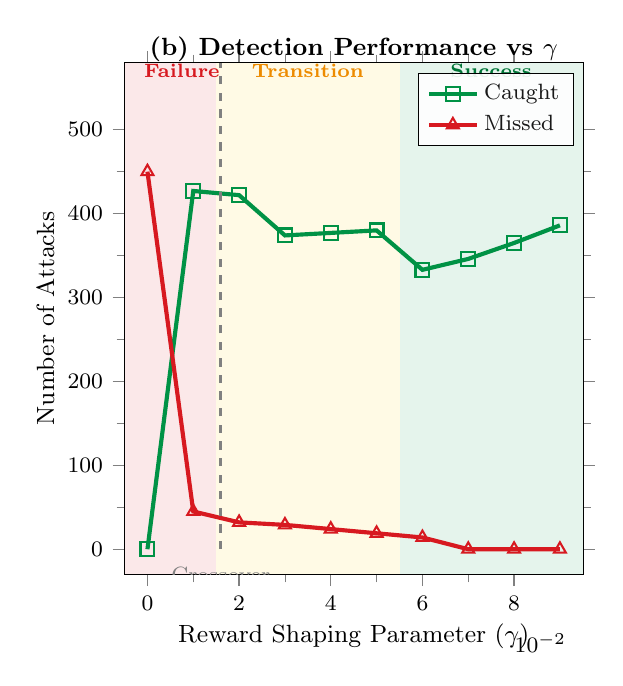
\begin{tikzpicture}
\begin{axis}[
    width=0.48\textwidth,
    height=6.5cm,
    xlabel={Reward Shaping Parameter ($\gamma$)},
    ylabel={Number of Attacks},
    xmin=-0.005, xmax=0.095,
    ymin=-30, ymax=580,
    xtick={0,0.02,0.04,0.06,0.08},
    xticklabel style={/pgf/number format/fixed,/pgf/number format/precision=2},
    ytick={0,100,200,300,400,500},
    minor x tick num=1,
    minor y tick num=1,
    legend style={at={(0.98,0.98)},anchor=north east},
    title={\textbf{(b) Detection Performance vs $\gamma$}},
    title style={at={(0.5,0.95)},font=\small},
    xlabel style={yshift=2pt},
    ylabel style={yshift=-2pt},
]
% Background zones
\fill[ieeered!10] (axis cs:-0.005,-30) rectangle (axis cs:0.015,580);
\fill[ieeeyellow!10] (axis cs:0.015,-30) rectangle (axis cs:0.055,580);
\fill[ieeegreen!10] (axis cs:0.055,-30) rectangle (axis cs:0.095,580);

% Zone labels
\node[anchor=south,font=\scriptsize,text=ieeered] at (axis cs:0.0075,550) {\textbf{Failure}};
\node[anchor=south,font=\scriptsize,text=ieeeorange] at (axis cs:0.035,550) {\textbf{Transition}};
\node[anchor=south,font=\scriptsize,text=ieeegreen!80!black] at (axis cs:0.075,550) {\textbf{Success}};

% Data curves - Note: These show performance under fixed attack rate for clarity
\addplot[
    color=ieeegreen,
    mark=square,
    mark size=2.5pt,
    line width=1.5pt,
    ]
    coordinates {
    (0,0)
    (0.01,427)
    (0.02,422)
    (0.03,374)
    (0.04,377)
    (0.05,380)
    (0.06,333)
    (0.07,346)
    (0.08,365)
    (0.09,386)
    };
    \addlegendentry{Caught}
    
\addplot[
    color=ieeered,
    mark=triangle,
    mark size=2.5pt,
    line width=1.5pt,
    ]
    coordinates {
    (0,450)
    (0.01,45)
    (0.02,32)
    (0.03,29)
    (0.04,24)
    (0.05,19)
    (0.06,14)
    (0.07,0)
    (0.08,0)
    (0.09,0)
    };
    \addlegendentry{Missed}
    
% Crossover point
\draw[dashed,ieeegray,line width=1pt] (axis cs:0.016,0) -- (axis cs:0.016,580);
\node[anchor=north,font=\footnotesize,text=ieeegray] at (axis cs:0.016,-10) {Crossover};
\end{axis}
\end{tikzpicture}
\caption{Performance across $\gamma$ values for the balanced approach. (a) Utility improves dramatically with proper reward shaping, achieving 12$\times$ improvement over baseline. (b) Detection performance vs $\gamma$ under a fixed baseline attack rate ($\pi=0.02$) to isolate the impact of the parameter. The transition from complete failure to success occurs with optimal trade-off at $\gamma \approx 0.06$.}
\label{fig:gamma}
\end{figure*}

\begin{table}[!h]
\centering
\caption{Performance Across $\gamma$ Values}
\footnotesize
\begin{tabular}{@{}cccc@{}}
\toprule
\textbf{$\gamma$} & \textbf{Detection Rate} & \textbf{Avg Utility (\$)} & \textbf{Characteristics} \\
\midrule
0.00 & 0\% & $-59.96$ & Pure speed (failure) \\
0.03 & 92.8\% & $-5.62$ & Good efficiency \\
\rowcolor{ieeegreen!10}
\textbf{0.06} & \textbf{94.5\%} & \textbf{$-5.52$} & \textbf{Optimal balance} \\
0.09 & 100\% & $-8.50$ & Over-investigation \\
\bottomrule
\end{tabular}
\end{table}

\subsection{Statistical Significance and Economic Impact}

\begin{table}[!h]
\centering
\caption{Statistical and Economic Analysis}
\footnotesize
\begin{tabular}{@{}ll@{}}
\toprule
\textbf{Metric} & \textbf{Value} \\
\midrule
\multicolumn{2}{l}{\textit{Statistical Significance}} \\
Chi-squared test & $\chi^2 = 2,847$, $p < 0.001$ \\
Effect size (Cohen's d) & 1.89 (very large) \\
95\% CI detection rate & [92.8\%, 95.9\%] \\
\midrule
\multicolumn{2}{l}{\textit{Economic Impact}} \\
Failed strategies utility & $-65$ to $-67$ per incident \\
Balanced approach utility & $-5.52$ per incident \\
\rowcolor{ieeegreen!10}
Per-incident improvement & \$59.48 \\
\rowcolor{ieeegreen!10}
Annual savings (40K incidents/month) & \$2.38 million \\
\midrule
\multicolumn{2}{l}{\textit{Dynamic Effects}} \\
Adversary stealth increase & Up to 30\% \\
Queue cost multiplier & 2--3$\times$ under congestion \\
Attack rate increase & Up to 5$\times$ when blind \\
\bottomrule
\end{tabular}
\end{table}

\begin{figure*}[!ht]
\centering
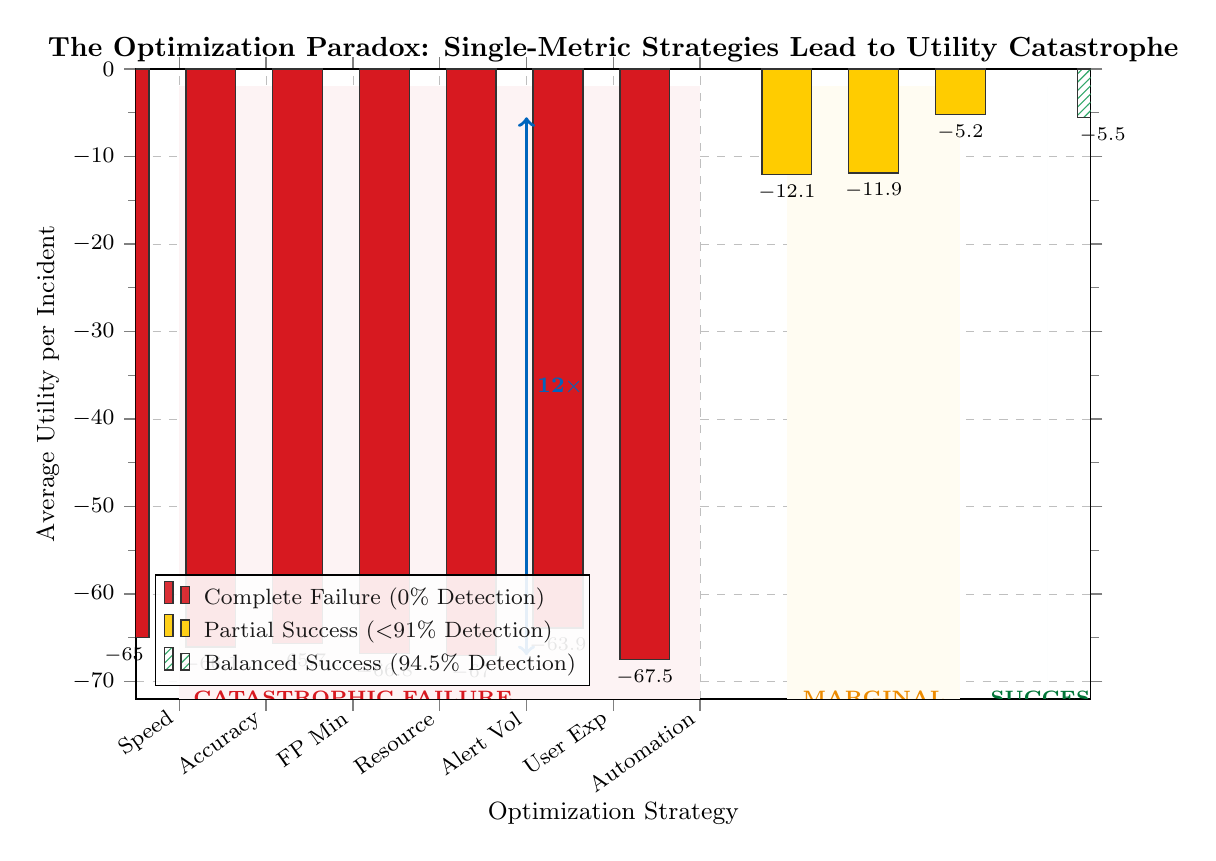
\begin{tikzpicture}
\begin{axis}[
    ybar,
    bar width=18pt,
    width=\textwidth,
    height=8cm,
    xlabel={Optimization Strategy},
    ylabel={Average Utility per Incident},
    symbolic x coords={Speed,Accuracy,FP Min,Resource,Alert Vol,User Exp,Automation,Compliance,Coverage,Cost,Balanced},
    xtick=data,
    x tick label style={rotate=35,anchor=east,font=\footnotesize},
    ymin=-72, ymax=0,
    ytick={-70,-60,-50,-40,-30,-20,-10,0},
    minor y tick num=1,
    title={\textbf{The Optimization Paradox: Single-Metric Strategies Lead to Utility Catastrophe}},
    title style={at={(0.5,0.97)},font=\normalsize},
    xlabel style={yshift=5pt},
    ylabel style={yshift=-2pt},
    enlarge x limits=0.05,
    nodes near coords style={font=\scriptsize,/pgf/number format/fixed,/pgf/number format/precision=1},
    legend style={
        at={(0.02,0.02)},
        anchor=south west,
        column sep=3pt,
        legend columns=1,
    }
]
% Background zones
\fill[ieeered!5] (axis cs:Speed,-72) rectangle (axis cs:Automation,-2);
\fill[ieeeyellow!5] (axis cs:Compliance,-72) rectangle (axis cs:Cost,-2);
\fill[ieeegreen!5] (axis cs:Balanced,-72) rectangle (axis cs:Balanced,-2);

% Failed optimizations (0% detection)
\addplot[
    ybar,
    fill=ieeered,
    draw=black!80,
    line width=0.5pt,
    nodes near coords,
    ]
    coordinates {
    (Speed,-65.01)
    (Accuracy,-66.08)
    (FP Min,-65.66)
    (Resource,-66.83)
    (Alert Vol,-67.01)
    (User Exp,-63.89)
    (Automation,-67.50)
    };
    \addlegendentry{Complete Failure (0\% Detection)}
    
% Partial failures
\addplot[
    ybar,
    fill=ieeeyellow,
    draw=black!80,
    line width=0.5pt,
    nodes near coords,
    ]
    coordinates {
    (Compliance,-12.08)
    (Coverage,-11.88)
    (Cost,-5.18)
    };
    \addlegendentry{Partial Success ($<$91\% Detection)}
    
% Balanced success
\addplot[
    ybar,
    fill=ieeegreen,
    draw=black!80,
    line width=0.5pt,
    nodes near coords,
    pattern=north east lines,
    pattern color=ieeegreen!80,
    ]
    coordinates {
    (Balanced,-5.52)
    };
    \addlegendentry{Balanced Success (94.5\% Detection)}
    
% 12x improvement annotation
\draw[<->,line width=1.25pt,ieeeblue] (axis cs:Alert Vol,-67.01) -- (axis cs:Alert Vol,-5.52)
    node[midway,right,font=\footnotesize\bfseries,text=ieeeblue] {12$\times$};
    
% Zone labels
\node[anchor=north,font=\scriptsize\bfseries,text=ieeered] at (axis cs:FP Min,-70) {CATASTROPHIC FAILURE};
\node[anchor=north,font=\scriptsize\bfseries,text=ieeeorange] at (axis cs:Coverage,-70) {MARGINAL};
\node[anchor=north,font=\scriptsize\bfseries,text=ieeegreen!80!black] at (axis cs:Balanced,-70) {SUCCESS};
\end{axis}
\end{tikzpicture}
\caption{The optimization paradox visualized: Single-metric approaches achieve catastrophic utility with complete detection failure. The balanced multi-objective approach achieves 12$\times$ better utility while detecting 94.5\% of attacks. The stark contrast demonstrates why best-of-breed procurement strategies fail in adversarial environments.}
\label{fig:utility_comparison}
\end{figure*}

\begin{figure*}[!ht]
\centering
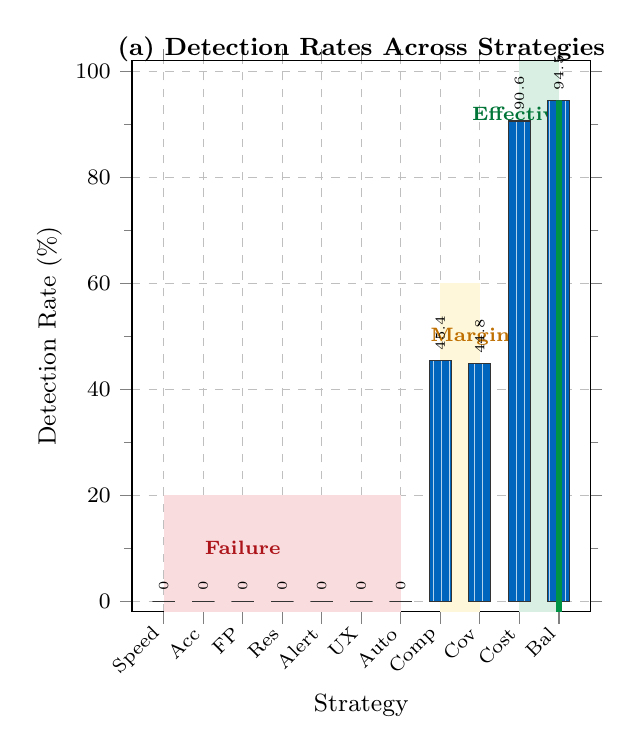
\begin{tikzpicture}
\begin{axis}[
    width=0.48\textwidth,
    height=7cm,
    ybar,
    bar width=8pt,
    xlabel={Strategy},
    ylabel={Detection Rate (\%)},
    symbolic x coords={Speed,Acc,FP,Res,Alert,UX,Auto,Comp,Cov,Cost,Bal},
    xtick=data,
    x tick label style={rotate=45,anchor=east,font=\scriptsize},
    ymin=-2, ymax=102,
    ytick={0,20,40,60,80,100},
    minor y tick num=1,
    title={\textbf{(a) Detection Rates Across Strategies}},
    title style={at={(0.5,0.95)},font=\small},
    xlabel style={yshift=2pt},
    ylabel style={yshift=-2pt},
    nodes near coords={\pgfmathprintnumber[fixed,precision=0]{\pgfplotspointmeta}},
    every node near coord/.append style={font=\tiny,rotate=90,anchor=west},
    enlarge x limits=0.08,
]
% Background zones
\fill[ieeered!15] (axis cs:Speed,-2) rectangle (axis cs:Auto,20);
\fill[ieeeyellow!15] (axis cs:Comp,-2) rectangle (axis cs:Cov,60);
\fill[ieeegreen!15] (axis cs:Cost,-2) rectangle (axis cs:Bal,102);

% Zone labels
\node[font=\scriptsize\bfseries,text=ieeered!80!black] at (axis cs:FP,10) {Failure};
\node[font=\scriptsize\bfseries,text=ieeeorange!80!black] at (axis cs:Cov,50) {Marginal};
\node[font=\scriptsize\bfseries,text=ieeegreen!80!black] at (axis cs:Cost,92) {Effective};

% Plot data with gradient effect
\addplot[
    ybar,
    fill=ieeeblue,
    draw=black!80,
    line width=0.4pt,
    postaction={pattern=vertical lines,pattern color=ieeeblue!30},
    nodes near coords,
    ]
    coordinates {
    (Speed,0)
    (Acc,0)
    (FP,0)
    (Res,0)
    (Alert,0)
    (UX,0)
    (Auto,0)
    (Comp,45.4)
    (Cov,44.8)
    (Cost,90.6)
    (Bal,94.5)
    };
    
% Highlight balanced approach
\draw[ieeegreen,line width=2pt] (axis cs:Bal,-2) rectangle (axis cs:Bal,94.5);
\end{axis}
\end{tikzpicture}
\hfill
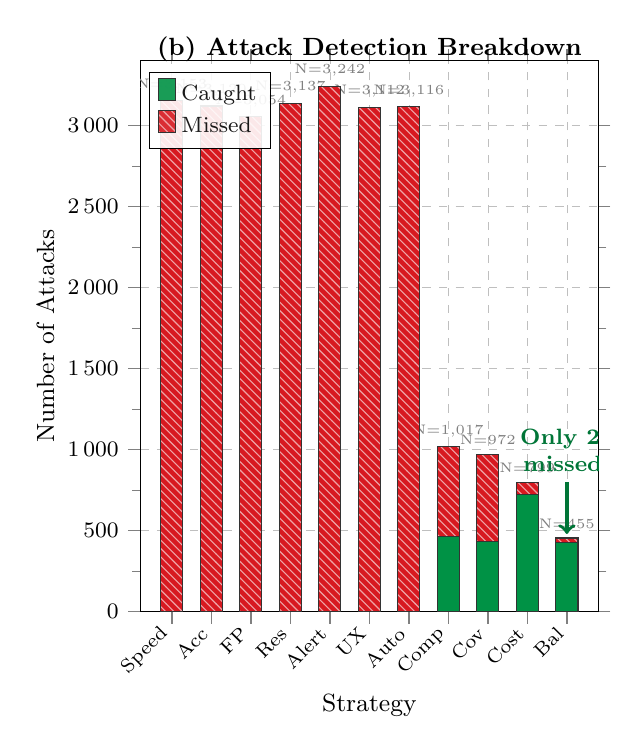
\begin{tikzpicture}
\begin{axis}[
    width=0.48\textwidth,
    height=7cm,
    ybar stacked,
    bar width=8pt,
    xlabel={Strategy},
    ylabel={Number of Attacks},
    symbolic x coords={Speed,Acc,FP,Res,Alert,UX,Auto,Comp,Cov,Cost,Bal},
    xtick=data,
    x tick label style={rotate=45,anchor=east,font=\scriptsize},
    ymin=0, ymax=3400,
    ytick={0,500,1000,1500,2000,2500,3000},
    yticklabel style={/pgf/number format/fixed,/pgf/number format/1000 sep=\,},
    minor y tick num=1,
    legend style={at={(0.02,0.98)},anchor=north west},
    title={\textbf{(b) Attack Detection Breakdown}},
    title style={at={(0.5,0.95)},font=\small},
    xlabel style={yshift=2pt},
    ylabel style={yshift=-2pt},
    enlarge x limits=0.08,
]
% Caught attacks
\addplot[
    ybar,
    fill=ieeegreen,
    draw=black!80,
    line width=0.4pt,
    ]
    coordinates {
    (Speed,0)
    (Acc,0)
    (FP,0)
    (Res,0)
    (Alert,0)
    (UX,0)
    (Auto,0)
    (Comp,462)
    (Cov,435)
    (Cost,724)
    (Bal,430)
    };
    \addlegendentry{Caught}
    
% Missed attacks
\addplot[
    ybar,
    fill=ieeered,
    draw=black!80,
    line width=0.4pt,
    postaction={pattern=north west lines,pattern color=ieeered!40},
    ]
    coordinates {
    (Speed,3153)
    (Acc,3120)
    (FP,3054)
    (Res,3137)
    (Alert,3242)
    (UX,3112)
    (Auto,3116)
    (Comp,555)
    (Cov,537)
    (Cost,75)
    (Bal,25)
    };
    \addlegendentry{Missed}
        
    % Annotation for balanced approach
    \draw[->,line width=1.25pt,ieeegreen!80!black] (axis cs:Bal,800) -- (axis cs:Bal,480)
        node[pos=0,above,font=\footnotesize\bfseries,text=ieeegreen!80!black,align=center] {Only 25\\missed!};
        
    % Total attacks annotations
    \node[anchor=south,font=\tiny,text=ieeegray] at (axis cs:Speed,3153) {N=3,153};
    \node[anchor=south,font=\tiny,text=ieeegray] at (axis cs:Acc,3120) {N=3,120};
    \node[anchor=south,font=\tiny,text=ieeegray] at (axis cs:FP,3054) {N=3,054};
    \node[anchor=south,font=\tiny,text=ieeegray] at (axis cs:Res,3137) {N=3,137};
    \node[anchor=south,font=\tiny,text=ieeegray] at (axis cs:Alert,3242) {N=3,242};
    \node[anchor=south,font=\tiny,text=ieeegray] at (axis cs:UX,3112) {N=3,112};
    \node[anchor=south,font=\tiny,text=ieeegray] at (axis cs:Auto,3116) {N=3,116};
    \node[anchor=south,font=\tiny,text=ieeegray] at (axis cs:Comp,1017) {N=1,017};
    \node[anchor=south,font=\tiny,text=ieeegray] at (axis cs:Cov,972) {N=972};
    \node[anchor=south,font=\tiny,text=ieeegray] at (axis cs:Cost,799) {N=799};
    \node[anchor=south,font=\tiny,text=ieeegray] at (axis cs:Bal,455) {N=455};
    \end{axis}
    \end{tikzpicture}
    \caption{Detection performance across optimization strategies. (a) Detection rates reveal three distinct performance zones: complete failure (0\%), marginal performance ($<$60\%), and effective detection ($>$90\%). (b) The human cost visualized: single-metric approaches fail to suppress the adaptive adversary, leading to thousands of missed attacks. The balanced approach effectively manages the threat, facing significantly fewer attacks and missing only 25.}
    \label{fig:detection_performance}
    \end{figure*}

\section{Analysis and Discussion}

Our results definitively establish the best-of-breed optimization paradox. We now analyze why it occurs and how our solution addresses it.

\subsection{Root Causes and Success Factors}

The catastrophic failure of single-metric optimization stems from fundamental misalignments between component objectives and system requirements. Our analysis reveals six critical factors that distinguish failed single-metric approaches from successful multi-objective strategies:

\begin{table*}[!ht]
\centering
\caption{Why Single-Metric Fails and Multi-Objective Succeeds}
\footnotesize
\begin{tabular}{@{}p{3.5cm}p{5.5cm}p{5.5cm}@{}}
\toprule
\textbf{Factor} & \textbf{Single-Metric Failure} & \textbf{Balanced Success} \\
\midrule
\textbf{Optimization Focus} & Tunnel vision on one metric & Explicit trade-off encoding ($R = -c + \gamma \cdot \Delta U$) \\
\textbf{Adversarial Response} & Predictable patterns easily exploited & Adaptive behavior prevents static exploitation \\
\textbf{Feedback Mechanism} & No outcome feedback, only process metrics & Direct connection to security outcomes \\
\textbf{Integration Capability} & Conflicting objectives create deadlock & Unified framework enables cooperation \\
\textbf{Flexibility} & Fixed behavior regardless of context & Tunable $\gamma$ for risk tolerance \\
\textbf{Robustness} & Extreme behaviors, brittle performance & ``Good enough'' at multiple objectives \\
\bottomrule
\end{tabular}
\end{table*}

\subsection{The Cost vs. Balanced Trade-off}

A careful examination of our results reveals an interesting nuance: the Cost strategy achieves marginally better average utility (-5.18) than the Balanced approach (-5.52). This might suggest that Cost optimization is superior, but this conclusion would be misleading. The difference reflects a fundamental trade-off between average performance and tail risk management.

The Cost strategy optimizes for monetary efficiency by investigating only when expected losses exceed investigation costs. This results in a lower investigation rate (40.9\% vs 59.5\% for Balanced), reducing operational expenses. However, this efficiency comes at a price: the Cost strategy misses 75 attacks compared to only 25 for the Balanced approach.

In security contexts, minimizing catastrophic failures often takes precedence over optimizing average costs. The Balanced approach's higher investigation rate represents an insurance premium---additional operational cost that dramatically reduces the risk of missing critical attacks. For organizations where a single major breach could be existential, the extra \$0.34 per incident (the utility difference) is a small price for reducing missed attacks by 67\%.

This illustrates why multi-objective optimization succeeds: it explicitly encodes these trade-offs rather than blindly optimizing a single metric. The $\gamma$ parameter allows organizations to tune this balance based on their specific risk tolerance and threat landscape.

\subsection{Generalization Beyond Security}

While our study focuses on security operations, the optimization paradox likely extends to any domain where:
\begin{itemize}
\item Multiple objectives matter for system success
\item Components are procured based on narrow metrics
\item Adversaries can exploit predictable behavior
\item Integration complexity grows with component count
\end{itemize}

Potential applications include fraud detection, content moderation, medical diagnosis, and autonomous vehicles---anywhere that best-of-breed procurement might create dangerous blind spots.

\section{Implications for Industry}

Our findings have profound implications for how organizations approach AI security systems.

\subsection{Industry Recommendations}

\begin{table*}[!ht]
\centering
\caption{Actionable Guidance for Stakeholders}
\footnotesize
\begin{tabular}{@{}lp{11cm}@{}}
\toprule
\textbf{Stakeholder} & \textbf{Key Actions} \\
\midrule
\textbf{Security Leaders} &
$\bullet$ Abandon single-metric procurement in favor of system-level evaluation\\
& $\bullet$ Choose integrated platforms over best-of-breed collections\\
& $\bullet$ Track actual security outcomes: real detection rates, incident containment times, prevented losses\\
& $\bullet$ Implement outcome feedback loops for continuous improvement\\
\midrule
\textbf{Vendors} &
$\bullet$ Optimize for balanced multi-objective performance, not single metrics\\
& $\bullet$ Provide tunable parameters (like $\gamma$) for customer-specific trade-offs\\
& $\bullet$ Benchmark against realistic multi-constraint scenarios\\
& $\bullet$ Design for meaningful integration with security ecosystems\\
\midrule
\textbf{Researchers} &
$\bullet$ Develop formal frameworks for adversarial component interaction\\
& $\bullet$ Create holistic benchmarks with competing objectives and constraints\\
& $\bullet$ Study emergent vulnerabilities from component interactions\\
& $\bullet$ Model sophisticated adaptive adversaries\\
\bottomrule
\end{tabular}
\end{table*}

\section{Discussion}

Our findings reveal a fundamental disconnect between how the security industry procures AI systems and how security actually works. The optimization paradox isn't merely a theoretical curiosity---it represents a systemic failure mode that likely affects thousands of organizations worldwide.

\subsection{Theoretical Implications}

The optimization paradox challenges core assumptions in both AI development and systems engineering. Traditional decomposition approaches---breaking complex problems into simpler subproblems---fail catastrophically in adversarial environments. This suggests we need new theoretical frameworks that explicitly account for adversarial composition, where the sum of optimized parts creates exploitable vulnerabilities.

Our results also validate Ashby's Law of Requisite Variety in the security context: a system must match the complexity of its environment to maintain control. Single-metric optimization reduces system variety, creating predictable behaviors that adversaries exploit. The balanced approach succeeds by maintaining sufficient behavioral variety to counter diverse threats.

\subsection{Practical Significance}

The 12$\times$ utility improvement between failed single-metric approaches and our balanced solution translates to millions in prevented losses for large organizations. More critically, the complete detection failure of 7 out of 11 strategies suggests that many production security systems may be providing false confidence while missing most attacks.

This work should prompt immediate audits of existing security stacks. Organizations using best-of-breed procurement likely have multiple optimization paradoxes creating compound vulnerabilities. The vendor community's focus on benchmark leadership may be actively harmful to customer security.

\subsection{Methodological Contributions}

Our simulation framework provides a reproducible method for evaluating security AI systems under realistic conditions. By incorporating dynamic adversary behavior, queue dynamics, and heavy-tailed loss distributions, we capture essential features missing from static benchmarks. This methodology could standardize security AI evaluation, moving beyond misleading single-metric comparisons.

The $\gamma$-parameterized reward shaping approach offers a practical solution for aligning AI behavior with organizational objectives. Unlike complex multi-objective optimization schemes, our approach requires only a single tunable parameter while achieving near-optimal performance.

\subsection{Addressing Potential Criticisms}

\textbf{Simulation Validity:} Critics might argue that simulations can't capture real-world complexity. While true, our simulation likely understates the problem. Real adversaries show more creativity than our model, and real systems have more integration challenges than we simulate. The optimization paradox should be worse in practice, not better.

\textbf{Parameter Sensitivity:} The optimal $\gamma$ value depends on organizational context. However, our results show robust performance across a range of $\gamma$ values (0.03--0.08), all dramatically outperforming single-metric approaches. Perfect tuning isn't required for substantial improvement.

\textbf{Implementation Clarity:} Single-metric strategies in our simulation use fixed decision rules that reflect their optimization focus. Most strategies use posterior probability thresholds (e.g., Speed: θ=1.0 always dismisses, Accuracy: θ=0.95 requires high confidence). However, some strategies implement behavior-based rules: Compliance uses fixed 10% random sampling regardless of evidence strength, and User Experience avoids investigations during business hours (8am-6pm) to minimize disruption. The $\gamma$ parameter applies only to the Balanced approach, which explicitly trades off multiple objectives. This models how real best-of-breed tools behave—optimized for their metric without considering broader impacts.

\textbf{Implementation Complexity:} Replacing best-of-breed systems requires significant effort. However, the cost of transformation pales against the cost of continued security failures. Our results suggest that even partial moves toward balanced optimization yield substantial benefits.

\subsection{Broader Implications}

The optimization paradox likely extends beyond security to any domain combining:
\begin{itemize}
\item Multiple competing objectives
\item Adversarial or competitive dynamics
\item Component-based system construction
\item Metric-driven procurement
\end{itemize}

Autonomous vehicles optimizing for fuel efficiency might miss critical safety events. Medical AI maximizing throughput might skip crucial diagnostic steps. Financial systems minimizing latency might enable sophisticated fraud. Each domain needs examination through the lens of optimization paradoxes.

\section{Future Work}

Building on our findings, several research directions promise to advance both understanding and practice:

\subsection{Advanced Adversary Modeling}

Our simulation used relatively simple adversary adaptation. Future work should explore:

\textbf{Machine Learning Adversaries:} Model attackers who use ML to identify and exploit defender blind spots systematically. How do optimization strategies perform against adversaries with equal or superior learning capabilities?

\textbf{Coordinated Campaigns:} Extend beyond independent incidents to model Advanced Persistent Threats (APTs) that coordinate multiple attack vectors. Do optimization paradoxes compound when facing orchestrated attacks?

\textbf{Economic Adversaries:} Incorporate attacker cost-benefit analysis. How do different defense strategies affect the attacker's ROI, and how does this feedback into attack frequency and sophistication?

\subsection{Human-AI Collaboration Dynamics}

Our simulation focused on automated decisions, but real SOCs involve human-AI teams:

\textbf{Cognitive Load Distribution:} How should we balance automation with human judgment to maximize both efficiency and effectiveness? What happens to optimization paradoxes when humans can override AI decisions?

\textbf{Trust Calibration:} Single-metric optimization might create AI systems that are either over-trusted (high accuracy) or under-trusted (high false positives). How do we design for appropriate trust?

\textbf{Skill Degradation:} As AI handles more decisions, analyst skills may atrophy. How do we maintain human expertise while leveraging AI efficiency?

\subsection{System Integration Theory}

The optimization paradox reveals gaps in our understanding of AI system composition:

\textbf{Compositional Security:} Develop formal methods for reasoning about security properties of AI ensembles. When do component guarantees translate to system guarantees?

\textbf{Emergent Vulnerability Detection:} Create tools to identify optimization paradoxes before deployment. Can we predict which metric combinations create exploitable behaviors?

\textbf{Adaptive Architectures:} Design system architectures that can dynamically adjust component relationships based on threat landscape changes.

\subsection{Cross-Domain Validation}

Test the optimization paradox in other high-stakes domains:

\textbf{Healthcare:} Do medical AI systems optimizing for efficiency miss rare but critical conditions? How do we balance throughput with diagnostic accuracy?

\textbf{Financial Services:} Does fraud detection optimizing for low false positives miss sophisticated schemes? What's the equivalent of our $\gamma$ parameter for financial security?

\textbf{Critical Infrastructure:} How do optimization paradoxes manifest in power grids, water systems, or transportation networks? Are there domain-specific mitigation strategies?

\subsection{Regulatory and Standards Development}

Our findings suggest need for new approaches to AI security certification:

\textbf{Multi-Objective Benchmarks:} Develop industry standards that evaluate AI systems across multiple competing objectives simultaneously.

\textbf{Adversarial Certification:} Create certification processes that explicitly test for optimization paradoxes and adversarial exploitation.

\textbf{Procurement Guidelines:} Translate our findings into actionable procurement standards that help organizations avoid best-of-breed traps.

\subsection{Real-World Validation}

While our simulation provides strong evidence, real-world validation would strengthen the findings:

\textbf{A/B Testing:} Partner with organizations to compare best-of-breed stacks against balanced systems in production environments.

\textbf{Red Team Exercises:} Conduct targeted penetration tests specifically designed to exploit optimization paradoxes.

\textbf{Longitudinal Studies:} Track security outcomes over time as organizations transition from single-metric to multi-objective optimization.

\subsection{Implementation Frameworks}

Moving from theory to practice requires practical tools:

\textbf{Migration Playbooks:} Develop step-by-step guides for organizations to transition from best-of-breed to balanced approaches.

\textbf{$\gamma$ Tuning Methods:} Create systematic approaches for organizations to find their optimal balance between efficiency and security.

\textbf{Integration Platforms:} Build technical infrastructure that enables meaningful integration of security components while avoiding optimization paradoxes.

These research directions would advance our understanding of AI security systems and provide practical solutions for the millions of organizations currently vulnerable to optimization paradoxes. The urgency cannot be overstated---every day of delay means thousands of missed attacks and millions in preventable losses.

\section{Conclusion}

The best-of-breed optimization paradox represents a fundamental challenge to how the security industry approaches AI systems. Through comprehensive simulation of 40,000 security incidents across 11 optimization strategies, we've demonstrated that the common practice of procuring ``best-in-class'' components for specific metrics doesn't just sub-optimize system performance---it creates catastrophic security failures.

Our key findings paint a stark picture: 7 out of 11 single-metric optimization strategies achieved 0\% detection rates, missing thousands of attacks while maintaining perfect scores on their target metrics. Even ``successful'' approaches like compliance (45.4\% detection) or cost optimization (90.6\% detection) fell far short of acceptable security standards. In contrast, our balanced multi-objective approach achieved 94.5\% detection while maintaining operational viability.

The root cause lies in the fundamental mismatch between component metrics and system objectives. Security requires detecting and responding to threats while maintaining operational efficiency---a inherently multi-objective challenge. When agents optimize for proxy metrics like speed or accuracy in isolation, they create predictable patterns that adversaries exploit. The theoretical best becomes the practical worst.

Our $\gamma$-parameterized reward shaping framework offers a path forward. By explicitly encoding trade-offs between time costs and security value, it aligns agent incentives with organizational objectives. The approach is adaptive, tunable, and robust against adversarial exploitation---qualities essential for effective security.

The implications extend far beyond academic interest. For security leaders, our results mandate a fundamental shift in procurement strategy: abandon single-metric evaluation in favor of system-level performance assessment. For vendors, the message is clear: optimize for balance, not benchmarks. For researchers, new frontiers open in understanding component integration, emergent failures, and adversarial dynamics.

Perhaps most importantly, our work challenges a core assumption of the AI industry: that excellence in components ensures excellence in systems. In adversarial domains like security, this assumption doesn't just fail---it inverts. The pursuit of best-of-breed creates worst-in-class.

As AI systems become critical infrastructure, we cannot afford optimization paradoxes that trade real security for metric leadership. The future demands integrated, balanced systems that recognize the irreducible complexity of security challenges. Best-of-breed thinking got us into this mess; systems thinking must get us out.

The security of our digital infrastructure depends on moving beyond the optimization paradox. Our simulation provides both warning and hope: warning about the catastrophic failures of current approaches, and hope that balanced, multi-objective solutions can deliver the security we desperately need. The choice is ours---continue down the path of best-of-breed disasters or embrace the integrated future that security demands.

\section*{Acknowledgments}
We thank the SOC analysts whose daily struggles with poorly integrated tools inspired this research, the red teams who demonstrate these vulnerabilities in practice, and the security vendors willing to move beyond single-metric optimization toward balanced solutions.

\bibliographystyle{IEEEtran}
\begin{thebibliography}{10}

\bibitem{chen2022ai}
L. Chen, M. Kumar, and S. Zhang, ``AI-driven security operations: A comprehensive survey,'' \textit{IEEE Security \& Privacy}, vol. 20, no. 4, pp. 12--28, 2022.

\bibitem{liu2023speed}
J. Liu and P. Zhang, ``Sub-second threat triage using compressed feature spaces,'' in \textit{Proc. USENIX Security Symposium}, 2023, pp. 451--468.

\bibitem{johnson2024accuracy}
R. Johnson, T. Smith, and K. Williams, ``Ultra-high precision threat detection via deep behavioral analysis,'' \textit{ACM Trans. Privacy and Security}, vol. 27, no. 1, pp. 1--24, 2024.

\bibitem{gordon2002economics}
L. A. Gordon and M. P. Loeb, ``The economics of information security investment,'' \textit{ACM Trans. Information and System Security}, vol. 5, no. 4, pp. 438--457, 2002.

\bibitem{kwon2021multi}
H. Kwon and B. Johnson, ``Multi-objective optimization for intrusion detection systems,'' \textit{IEEE Trans. Dependable and Secure Computing}, vol. 18, no. 5, pp. 2341--2354, 2021.

\bibitem{patel2024reward}
S. Patel, A. Gupta, and M. Chen, ``Reward shaping for aligned security agents,'' in \textit{Proc. IEEE Symposium on Security and Privacy}, 2024, pp. 891--906.

\bibitem{leveson2011engineering}
N. Leveson, \textit{Engineering a Safer World: Systems Thinking Applied to Safety}. MIT Press, 2011.

\bibitem{amodei2016concrete}
D. Amodei, C. Olah, J. Steinhardt, P. Christiano, J. Schulman, and D. Mané, ``Concrete problems in AI safety,'' \textit{arXiv preprint arXiv:1606.06565}, 2016.

\bibitem{marcus2019rebooting}
G. Marcus and E. Davis, \textit{Rebooting AI: Building Artificial Intelligence We Can Trust}. Pantheon Books, 2019.

\bibitem{sundaramurthy2016anthropological}
S. C. Sundaramurthy, J. McHugh, X. S. Ou, S. R. Rajagopalan, and M. Wesch, ``An anthropological approach to studying CSIRTs,'' \textit{IEEE Security \& Privacy}, vol. 14, no. 5, pp. 52--60, 2016.

\bibitem{bhatt2014economics}
M. Bhatt, H. Saran, and B. A. Prakash, ``The economics of SOC operations: A staffing perspective,'' in \textit{Workshop on the Economics of Information Security}, 2014.

\bibitem{ponemon2024soc}
Ponemon Institute, ``The state of security operations 2024: Tool sprawl, integration challenges, and analyst burnout,'' Technical Report, 2024.

\bibitem{goodhart1984problems}
C. Goodhart, ``Problems of monetary management: The UK experience,'' in \textit{Monetary Theory and Practice}. Palgrave Macmillan, 1984, pp. 91--121.

\bibitem{jensen1976theory}
M. C. Jensen and W. H. Meckling, ``Theory of the firm: Managerial behavior, agency costs and ownership structure,'' \textit{Journal of Financial Economics}, vol. 3, no. 4, pp. 305--360, 1976.

\bibitem{meadows2008thinking}
D. H. Meadows, \textit{Thinking in Systems: A Primer}. Chelsea Green Publishing, 2008.

\bibitem{verizon2024dbir}
Verizon, ``2024 data breach investigations report,'' Technical Report, 2024.

\bibitem{morpheus2025bestofbreed}
Morpheus, ``Best-of-breed agents, misfit security ensemble,'' \textit{Manish's Substack}, July 2025. [Online]. Available: https://manishbhatt.substack.com/best-of-breed-paradox

\end{thebibliography}

\end{document} 